\chapter{Założenia projektowe}
\section{Wymagania funkcjonalne}


\begin{minipage}{\textwidth}
    \begin{table}[H]
        \centering\caption{Wymagania funkcjonalne ogólne (opr.wł)\label{tabela:wymaganiaFunkcjonalneOgolne}}
        \begin{tabular}{|p{.3\textwidth}|p{.6\textwidth}|}
            \hline
            Potrzeby & Cechy \\

            \hline
            Administrator potrzebuje widzieć listę użytkowników &
            \begin{itemize}
                \item Przydzielanie i odbieranie użytkownikom uprawnień
            \end{itemize} \\
            \hline
        \end{tabular}
    \end{table}
\end{minipage}

\begin{minipage}{\textwidth}
    \begin{table}[H]
        \centering\caption{Wymagania funkcjonalne dla produktów (opr.wł)\label{tabela:wymaganiaFunkcjonalneProdukty}}
        \begin{tabular}{|p{.3\textwidth}|p{.6\textwidth}|}
            \hline
            Potrzeby & Cechy \\

            \hline
            Administrator potrzebuje zarządzać definicjami potrzebnymi w produktach &
            \begin{itemize}
                \item Zarządzanie definicjami wartości odżywczych
                \item Zarządzanie kategoriami produktów
                \item Zarządzanie rodzajami diet
            \end{itemize} \\
            \hline
            Dietetyk potrzebuje widzieć listę produktów &
            \begin{itemize}
                \item Wyszukiwanie produktów
                \item Filtrowanie produktów
                \item Dodawanie nowych produktów
            \end{itemize} \\
            \hline
            Dietetyk potrzebuje zarządzać szczegółami produktu &
            \begin{itemize}
                \item Edytowanie i usuwanie produktów
                \item Definiowanie wartości odżywczych dla produktu
                \item Definiowanie miar domowych dla produktu
                \item Przypisywanie produktu do kategorii i podkategorii
                \item Definiowanie do jakich typów diet produkt nadaje się a do jakich nie
            \end{itemize} \\
            \hline
        \end{tabular}
    \end{table}
\end{minipage}

\begin{minipage}{\textwidth}
    \begin{table}[H]
        \centering\caption{Wymagania funkcjonalne dla przepisów (opr.wł)\label{tabela:wymaganiaFunkcjonalnePrzepisy}}
        \begin{tabular}{|p{.3\textwidth}|p{.6\textwidth}|}
            \hline
            Potrzeby & Cechy \\

            \hline
            Administrator potrzebuje zarządzać definicjami potrzebnymi w przepisach &
            \begin{itemize}
                \item Zarządzanie typami posiłków
                \item Zarządzanie typami dań
                \item Zarządzanie definicjami wyposażenia kuchennego
            \end{itemize} \\
            \hline
            Dietetyk potrzebuje widzieć listę przepisów &
            \begin{itemize}
                \item Wyszukiwanie przepisów
                \item Filtrowanie przepisów
                \item Dodawanie nowych przepisów
            \end{itemize} \\
            \hline
            Dietetyk potrzebuje zarządzać szczegółami przepisu &
            \begin{itemize}
                \item Edytowanie i usuwanie przepisów
                \item Dodawanie wielu sekcji do przepisu
                \item Dodawanie do każdej sekcji listy składników
                \item Dodawanie do każdej sekcji sposobu przygotowania
                \item Dodawanie zdjęcia dania do przepisu
                \item Definiowanie czasu przygotowania posiłku
            \end{itemize} \\
            \hline
        \end{tabular}
    \end{table}
\end{minipage}

\begin{minipage}{\textwidth}
    \begin{table}[H]
        \centering\caption{Wymagania funkcjonalne dla jadłospisów (opr.wł)\label{tabela:wymaganiaFunkcjonalneJadlospisy}}
        \begin{tabular}{|p{.3\textwidth}|p{.6\textwidth}|}
            \hline
            Potrzeby & Cechy \\

            \hline
            Dietetyk potrzebuje widzieć listę jadłospisów &
            \begin{itemize}
                \item Wyszukiwanie jadłospisów
                \item Filtrowanie jadłospisów
                \item Dodawanie nowych jadłospisów
            \end{itemize} \\
            \hline
            Dietetyk potrzebuje zarządzać szczegółami jadłospisu &
            \begin{itemize}
                \item Dodawanie, edytowanie i usuwanie jadłospisów
                \item Definiowanie liczby dni na które będzie układany jadłospis
                \item Definiowanie liczby posiłków dziennie
                \item Definiowanie planowanego czasu każdego z posiłków
                \item Definiowanie procentowego udziału podstawowych wartości odżywczych w każdym posiłku
                \item Definiowanie posiłków w jadłospisie
                \item Dodawanie produktów i przepisów do posiłków
            \end{itemize} \\
            \hline
        \end{tabular}
    \end{table}
\end{minipage}

\begin{minipage}{\textwidth}
    \begin{table}[H]
        \centering\caption{Wymagania funkcjonalne dla wizyt (opr.wł)\label{tabela:wymaganiaFunkcjonalneWizyty}}
        \begin{tabular}{|p{.3\textwidth}|p{.6\textwidth}|}
            \hline
            Potrzeby & Cechy \\

            \hline
            Dietetyk potrzebuje wyświetlać listę swoich pacjentów &
            \begin{itemize}
                \item Wyszukiwanie pacjentów
                \item Wyświetlanie listy znalezionych pacjentów
                \item Wyświetlanie listy umówionych wizyt
                \item Wyświetlanie listy oczekujących porad
                \item Dodawanie nowych pacjentów
            \end{itemize} \\
            \hline
            Dietetyk potrzebuje zarządzać kartą pacjenta &
            \begin{itemize}
                \item Wyświetlanie i edytowanie podstawowych informacji pacjenta
                \item Wyświetlanie listy wizyt pacjenta
                \item Wyświetlanie listy oczekujących porad pacjenta
                \item Dodawanie nowej wizyty pacjenta
            \end{itemize} \\
            \hline
            Dietetyk potrzebuje wyświetlać szczegóły wizyty pacjenta &
            \begin{itemize}
                \item Wyświetlanie i edytowanie szczegółów wizyty pacjenta
                \item Zarządzanie pomiarami ciała pacjenta przypisanymi do wizyty
                \item Zarządzanie wywiadem żywieniowym przypisanym do wizyty
                \item Zarządzanie jadłospisem przydzielonym do wizyty
            \end{itemize} \\
            \hline
            Pacjent potrzebuje otrzymywać dietę &
            \begin{itemize}
                \item Automatyczne wysyłanie do pacjenta diety mailem po zatwierdzeniu jadłospisu przez dietetyka
            \end{itemize} \\
            \hline
            Pacjent chce mieć wgląd w swoją kartę &
            \begin{itemize}
                \item Logowanie do konta utworzonego w serwisie
                \item Dodawanie kart pacjenta do swojego konta po udostępnieniu ich przez dietetyka
            \end{itemize} \\
            \hline
            Pacjent zarządza dietą za pomocą asystenta głosowego &
            \begin{itemize}
                \item Wydawanie w języku naturalnym poleceń dotyczących diety
            \end{itemize} \\
            \hline
        \end{tabular}
    \end{table}
\end{minipage}

\newpage
\section{Wymagania niefunkcjonalne}
\begin{itemize}
    \item System działa poprawnie w przeglądarce Google Chrome i Firefox
    \item System działa poprawnie w przeglądarce Edge i Opera
    \item System działa poprawnie w przeglądarce Internet Explorer i Safari
    \item System działa na urządzenia mobilnych Android
    \item System działa na urządzeniach mobilnych iOS
    \item System jest dostępny w polskiej wersji językowej
    \item System ma czytelny i ładny interfejs
    \item Aplikacja webowa jest w pełni responsywna i wygodna do używania niezależnie od wielkości ekranu urządzenia klienckiego
    \item Aplikacja webowa udostępnia część funkcji offline
    \item Aplikacja ma być oparta na architekturze mikroserwisów
\end{itemize}

\section{Ograniczenia dziedzinowe}

\section{Model domenowy}


\begin{minipage}{\textwidth}
    \begin{figure}[H]
        \centering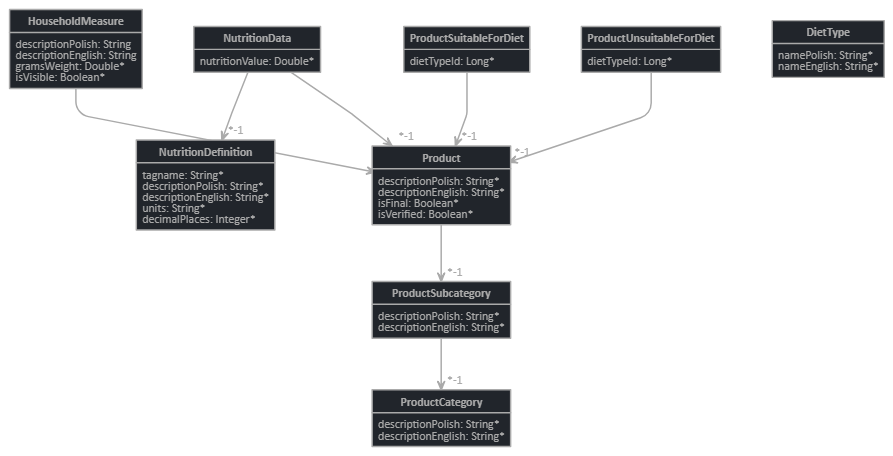
\includegraphics[width=0.9\textwidth]{img/class-diagrams/produkty.png}
        \caption{Produkty (opr.wł).}\label{rysunek:produkty}
    \end{figure}
\end{minipage}

\begin{minipage}{\textwidth}
    \begin{figure}[H]
        \centering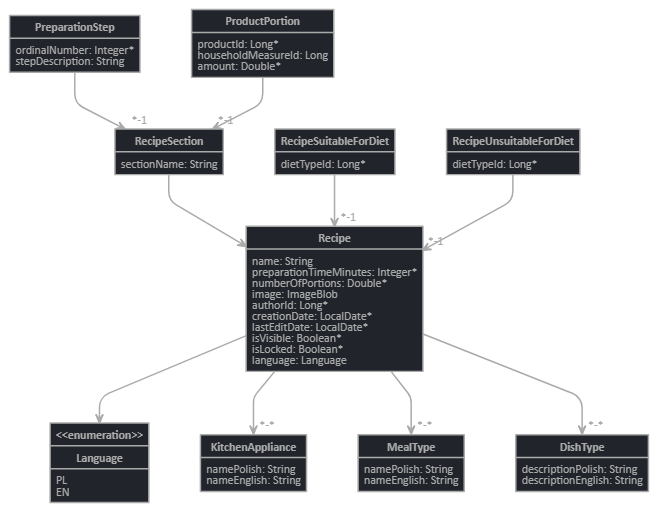
\includegraphics[width=0.9\textwidth]{img/class-diagrams/przepisy.png}
        \caption{Przepisy (opr.wł).}\label{rysunek:przepisy}
    \end{figure}
\end{minipage}

\begin{minipage}{\textwidth}
    \begin{figure}[H]
        \centering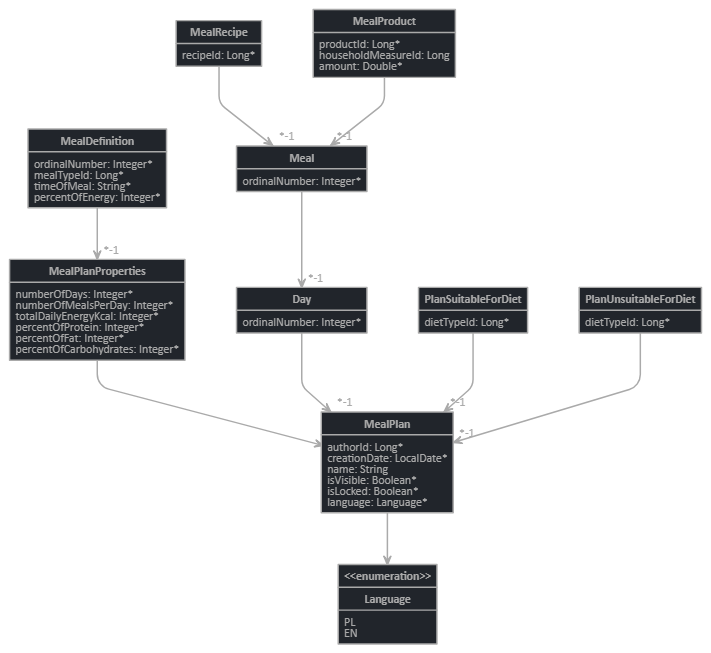
\includegraphics[width=0.9\textwidth]{img/class-diagrams/jadospisy.png}
        \caption{Jadłospisy (opr.wł).}\label{rysunek:jadlospisy}
    \end{figure}
\end{minipage}

\begin{minipage}{\textwidth}
    \begin{figure}[H]
        \centering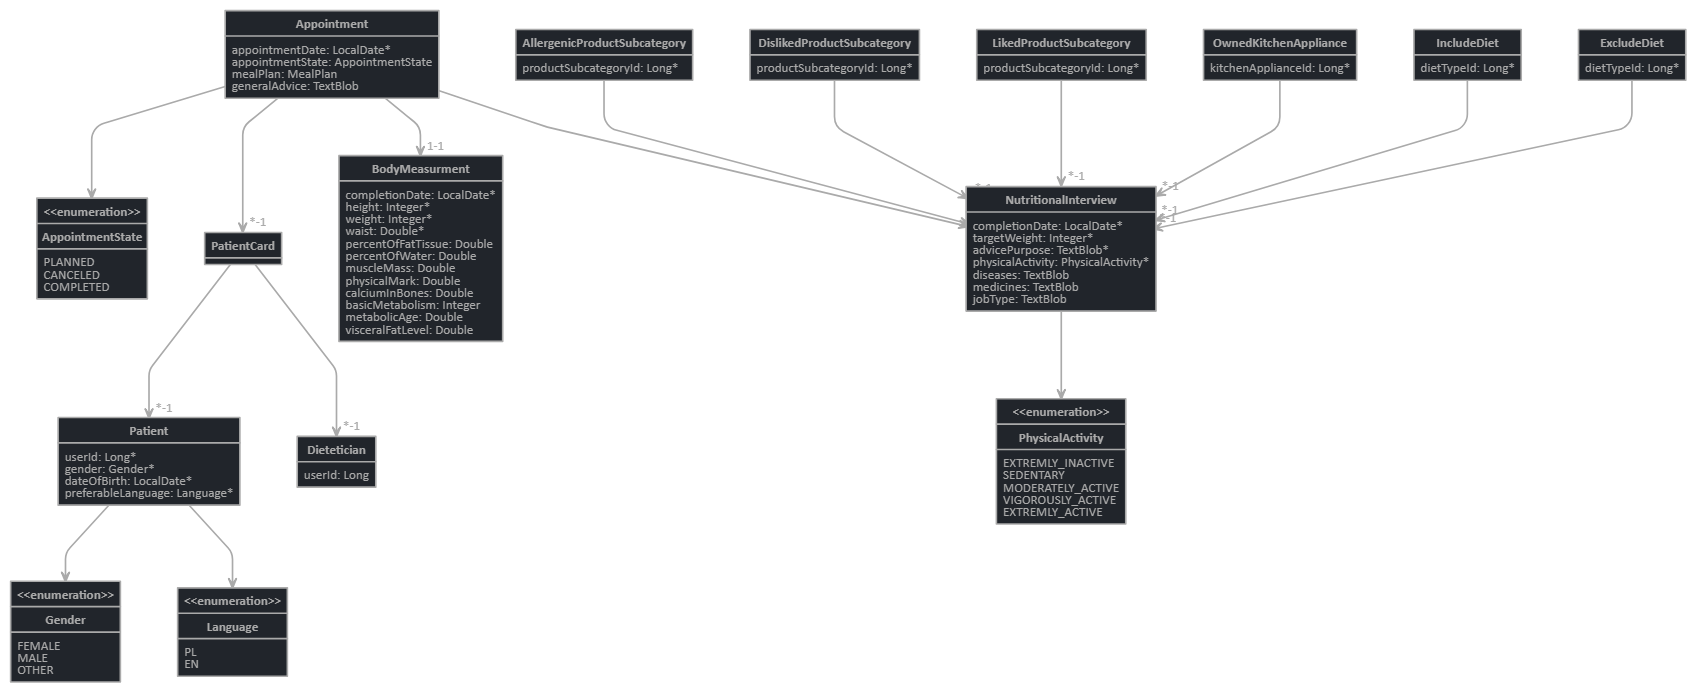
\includegraphics[width=0.9\textwidth]{img/class-diagrams/wizyty.png}
        \caption{Wizyty (opr.wł).}\label{rysunek:wizyty}
    \end{figure}
\end{minipage}

\thispagestyle{normal}
